\documentclass[tikz,border=2pt]{standalone}
\usepackage{amsmath}
\usepackage{pgfplots}
\pgfplotsset{compat=1.18}

\begin{document}
% lim_{x->a} f(x) = L for f(x)=(x^2-1)/(x-1), a=1, L=2: the value f(1) does not exist (hole),
% yet for every band L±ε there is an interval a±δ whose points (other than a) land in the band.
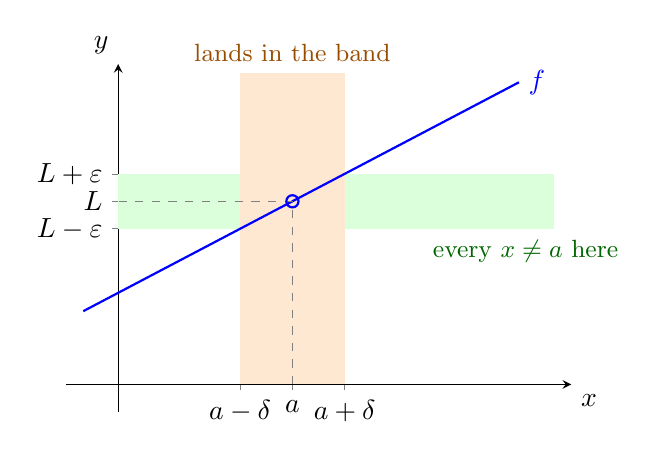
\begin{tikzpicture}
	\begin{axis}[
		axis lines=middle,
		xmin=-0.3, xmax=2.6,
		ymin=-0.3, ymax=3.5,
		xtick={0.7,1,1.3}, xticklabels={$a-\delta$,$a$,$a+\delta$},
		ytick={1.7,2,2.3}, yticklabels={$L-\varepsilon$,$L$,$L+\varepsilon$},
		xlabel={$x$}, ylabel={$y$},
		xlabel style={below right}, ylabel style={above left},
		samples=2, clip=false,
		width=8cm, height=6cm
		]
		\fill[green!14] (axis cs:0,1.7) rectangle (axis cs:2.5,2.3);
		\fill[orange!18] (axis cs:0.7,0) rectangle (axis cs:1.3,3.4);
		\addplot[thick, blue, domain=-0.2:2.3] {x+1};
		\addplot[only marks, mark=o, mark size=2.2pt, blue, thick, fill=white] coordinates {(1,2)};
		\draw[dashed, gray] (axis cs:1,0) -- (axis cs:1,2) -- (axis cs:0,2);
		\node[green!40!black, anchor=west, font=\small] at (axis cs:1.75,1.45) {every $x\neq a$ here};
		\node[orange!60!black, anchor=south, font=\small] at (axis cs:1,3.42) {lands in the band};
		\node[blue, anchor=west] at (axis cs:2.3,3.3) {$f$};
	\end{axis}
\end{tikzpicture}
\end{document}
